\section{Serial Data Transfer - SPI}

\subsection{Serial Communication Basics}

\begin{concept}{Serial vs. Parallel Communication}\\
Microcontrollers often use serial connections for communication:
\begin{itemize}
    \item \textbf{Serial Connection}: Data transmitted one bit at a time over fewer wires
    \begin{itemize}
        \item Simpler (saves PCB area)
        \item Reduces number of switching lines (reduced power, improved EMC)
        \item Requires higher-level protocol for interpretation
    \end{itemize}
    \item \textbf{Parallel Bus}: Data transmitted over multiple lines simultaneously
    \begin{itemize}
        \item Faster for short distances
        \item More complex routing
        \item Higher power consumption and EMC issues
    \end{itemize}
\end{itemize}
\end{concept}

\begin{definition}{Serial Communication Modes}
\begin{itemize}
    \item \textbf{Simplex}: Unidirectional, one-way only communication
    \item \textbf{Half-duplex}: Bidirectional, but only one direction at a time
    \item \textbf{Full-duplex}: Bidirectional, both directions simultaneously
\end{itemize}
\end{definition}

\begin{definition}{Serial Communication Timing}
\begin{itemize}
    \item \textbf{Synchronous}: Both nodes use the same clock
    \begin{itemize}
        \item Clock often provided by master
        \item Examples: SPI, I2C
    \end{itemize}
    \item \textbf{Asynchronous}: Each node uses an individual clock
    \begin{itemize}
        \item Start/stop bits used for synchronization
        \item Example: UART
    \end{itemize}
\end{itemize}
\end{definition}

\subsection{SPI Overview}

\begin{concept}{SPI - Serial Peripheral Interface}\\
SPI is a synchronous serial bus primarily for on-board connections:
\begin{itemize}
    \item Introduced by Motorola (now NXP) around 1979
    \item Also called 4-wire bus
    \item De facto standard (no legally binding specification)
    \item Used for short-distance communication
    \item Connects microcontroller to external devices (sensors, displays, flash memory, etc.)
    \item Full-duplex communication
    \item Single master, multiple slaves
    \item Synchronous (master provides clock)
\end{itemize}
\end{concept}

\begin{definition}{SPI Signals}
\begin{itemize}
    \item \textbf{SCLK} (Serial Clock): Generated by master
    \item \textbf{MOSI} (Master Out Slave In): Data from master to slave
    \item \textbf{MISO} (Master In Slave Out): Data from slave to master
    \item \textbf{SS/CS} (Slave Select/Chip Select): Enables specific slave(s)
\end{itemize}
\end{definition}

\begin{concept}{SPI Master-Slave Architecture}
\begin{itemize}
    \item Master generates common clock signal (SCLK) for all slaves
    \item Master selects slave by asserting the appropriate SS line (active low)
    \item MOSI line connects to inputs of all slaves
    \item MISO lines from all slaves are connected to a single master input
    \item Inactive slaves (SS = '1') put their MISO line in tri-state (high impedance)
    \item Only one selected slave drives its MISO line at a time
\end{itemize}
\end{concept}

\subsection{SPI Implementation}

\begin{concept}{SPI Implementation Using Shift Registers}
\begin{itemize}
    \item Both master and slave contain 8-bit shift registers
    \item Bits are shifted out on one clock edge (toggling edge)
    \item Bits are sampled on the other clock edge (sampling edge)
    \item 8 clock cycles exchange 8 bits in each direction simultaneously
    \item After 8 clock cycles, data has been exchanged in both directions
    \item Status flags (TXE, RXNE) indicate buffer status
\end{itemize}
\end{concept}

\subsection{SPI Modes}

\begin{concept}{Clock Polarity and Phase}
SPI has four different modes based on two parameters:
\begin{itemize}
    \item \textbf{CPOL} (Clock Polarity): Idle state of clock
    \begin{itemize}
        \item CPOL = 0: Clock idles at low level
        \item CPOL = 1: Clock idles at high level
    \end{itemize}
    \item \textbf{CPHA} (Clock Phase): Which edge is used for data sampling
    \begin{itemize}
        \item CPHA = 0: Data sampled on first clock edge
        \item CPHA = 1: Data sampled on second clock edge
    \end{itemize}
\end{itemize}
\end{concept}

\begin{concept}{Four SPI Modes}
\begin{itemize}
    \item \textbf{Mode 0}: CPOL = 0, CPHA = 0
    \begin{itemize}
        \item Clock idles low
        \item Data sampled on rising edge, changed on falling edge
    \end{itemize}
    \item \textbf{Mode 1}: CPOL = 0, CPHA = 1
    \begin{itemize}
        \item Clock idles low
        \item Data sampled on falling edge, changed on rising edge
    \end{itemize}
    \item \textbf{Mode 2}: CPOL = 1, CPHA = 0
    \begin{itemize}
        \item Clock idles high
        \item Data sampled on falling edge, changed on rising edge
    \end{itemize}
    \item \textbf{Mode 3}: CPOL = 1, CPHA = 1
    \begin{itemize}
        \item Clock idles high
        \item Data sampled on rising edge, changed on falling edge
    \end{itemize}
\end{itemize}
\end{concept}

\subsection{SPI Characteristics}

\begin{definition}{SPI Properties}
\begin{itemize}
    \item No defined addressing scheme (uses SS lines instead)
    \item No built-in acknowledgment or error detection
    \item Originally for single-byte transfers (now also used for streaming)
    \item Flexible data rate (clock signal is transmitted with data)
    \item No flow control (master controls timing, slave cannot influence)
    \item Susceptible to clock line noise
\end{itemize}
\end{definition}

\columnbreak

\subsection{STM32 SPI Implementation}

\begin{concept}{STM32 SPI Architecture}
The STM32F4 SPI peripheral includes:
\begin{itemize}
    \item Configuration registers (SPI\_CR1, SPI\_CR2)
    \item Status register (SPI\_SR)
    \item Data register (SPI\_DR) for transmit and receive
    \item Status flags for synchronization (TXE, RXNE, BSY)
    \item Support for different communication modes
    \item DMA capability for high-speed transfers
\end{itemize}
\end{concept}

\begin{code}{STM32 SPI Register Configuration}
\begin{lstlisting}[language=C, style=basesmol]
// SPI configuration example
// Configure SPI1 in master mode, CPOL=1, CPHA=1, 8-bit data

// Enable SPI1 clock
RCC->APB2ENR |= RCC_APB2ENR_SPI1EN;

// Configure SPI1
SPI1->CR1 = (1 << 0)   // CPHA=1
          | (1 << 1)   // CPOL=1
          | (1 << 2)   // Master mode
          | (3 << 3)   // BR[2:0]=011: fPCLK/16 (prescaler)
          | (0 << 7)   // MSB first (LSBFIRST=0)
          | (1 << 8)   // SSI=1 (needed for software SS)
          | (1 << 9);  // SSM=1 (software slave management)

// Enable SPI
SPI1->CR1 |= (1 << 6); // SPE=1 (SPI enable)
\end{lstlisting}
\end{code}

\begin{KR}{Transmitting Data with SPI}
\paragraph{Step 1: Prepare SPI}
Configure and enable the SPI peripheral.
\paragraph{Step 2: Check TXE flag}
Wait until the transmit buffer is empty.
\paragraph{Step 3: Write data}
Write data to the data register.
\paragraph{Step 4: Wait for completion}
Wait until transmission is complete by checking BSY flag.

\begin{lstlisting}[language=C, style=basesmol]
// Transmit a byte over SPI
uint8_t transmit_byte(uint8_t data) {
    // Step 1: SPI should already be configured
    
    // Step 2: Wait until TXE=1 (transmit buffer empty)
    while (!(SPI1->SR & (1 << 1))) { }
    
    // Step 3: Write data to transmit
    SPI1->DR = data;
    
    // Step 4: Wait for reception (needed to get received data)
    while (!(SPI1->SR & (1 << 0))) { }
    
    // Return received data (read DR clears RXNE flag)
    return SPI1->DR;
}
\end{lstlisting}
\end{KR}

\begin{KR}{Handling Full-Duplex SPI Communication}
\paragraph{Step 1: Enable SPI with SPE bit}
Ensure SPI is properly configured and enabled.
\paragraph{Step 2: Write first byte to transmit}
Write the first byte to DR to start transmission/reception.
\paragraph{Step 3: Process data in a loop}
Check TXE and RXNE flags to handle both transmission and reception.
\paragraph{Step 4: Wait for completion}
Wait for BSY=0 to ensure all transfers are complete.

\begin{lstlisting}[language=C, style=basesmol]
// Full-duplex SPI communication
void spi_transfer(uint8_t *tx_data, uint8_t *rx_data, uint16_t length) {
    // Enable SPI
    SPI1->CR1 |= (1 << 6);  // SPE=1
    
    // Write first TX byte to start transmission
    if (length > 0) {
        SPI1->DR = tx_data[0];
    }
    
    uint16_t tx_count = 1;
    uint16_t rx_count = 0;
    
    // Process data
    while (rx_count < length) {
        // Check if we can transmit more data
        if ((tx_count < length) && (SPI1->SR & (1 << 1))) {  // TXE=1
            SPI1->DR = tx_data[tx_count++];
        }
        
        // Check if we received data
        if (SPI1->SR & (1 << 0)) {  // RXNE=1
            rx_data[rx_count++] = SPI1->DR;
        }
    }
    
    // Wait until BSY=0 (SPI not busy)
    while (SPI1->SR & (1 << 7)) { }
}
\end{lstlisting}
\end{KR}

\begin{example2}{SPI Mode Identification from Timing Diagram}\\
Given the following timing diagram, identify the SPI mode (CPOL/CPHA values):
\important{add actual timing diagram here}\\
%SCLK: \_/‾\\\_/‾\\\_/‾\\\_/‾\\\_/‾\\\_/‾\\\_/‾\\\_/‾\\\_
%MOSI: ‾‾\\\_\_\_/‾‾‾\\\_\_\_/‾‾‾\\\_\_\_/‾‾‾
Data:  1     0     1     0     1     1     0     1

\tcblower
Looking at the diagram:
- Clock starts low and returns to low between transfers (CPOL = 0)
- Data appears to change on rising edges
- Data is sampled on falling edges

This corresponds to Mode 1: CPOL = 0, CPHA = 1
\end{example2}

\raggedcolumns
\pagebreak

\section{Serial Data Transfer - UART \& I2C}

\subsection{UART Fundamentals}

\mult{2}

\begin{concept}{UART - Universal Asynchronous Receiver Transmitter}\\
UART is an asynchronous serial communication interface:
\begin{itemize}
    \item Asynchronous - no shared clock between transmitter and receiver
    \item Point-to-point communication (one transmitter, one receiver)
    \item Full-duplex (simultaneous bidirectional communication)
    \item Start and stop bits used for synchronization
    \item Typically 2-wire interface (TX and RX) for data
    \item Optional control signals (RTS/CTS, etc.) for flow control
\end{itemize}
\end{concept}

\begin{definition}{UART Signals}\\
Basic UART connections require:
\begin{itemize}
    \item \textbf{TX} (Transmit): Data output from transmitter to receiver
    \item \textbf{RX} (Receive): Data input from transmitter to receiver
    \item \textbf{GND} (Ground): Common reference level
\end{itemize}
Extended UART (with hardware flow control) may include:
\begin{itemize}
    \item \textbf{RTS} (Request to Send): Output indicating readiness to receive
    \item \textbf{CTS} (Clear to Send): Input indicating partner is ready to receive
\end{itemize}
\end{definition}

\multend

\subsection{UART Data Format and Timing}

\mult{2}

\begin{definition}{UART Frame Structure}\\
A UART frame consists of:
\begin{itemize}
    \item \textbf{Idle state}: Line is high ('1') when no transmission occurs
    \item \textbf{Start bit}: Always '0', indicates beginning of frame
    \item \textbf{Data bits}: 5 to 9 bits (typically 8), LSB first
    \item \textbf{Parity bit} (optional): For error detection
    \item \textbf{Stop bit(s)}: 1, 1.5, or 2 bits, always '1'
\end{itemize}
\end{definition}

\begin{concept}{UART Synchronization}\\
Without a common clock, UART devices synchronize as follows:
\begin{itemize}
    \item Receiver detects start bit (falling edge from idle to '0')
    \item Receiver samples middle of each bit based on configured baud rate
    \item Both devices must use the same configuration:
    \begin{itemize}
        \item Baud rate (e.g., 9600, 115200 bits/s)
        \item Number of data bits (5-8)
        \item Parity (none, odd, even, mark, space)
        \item Number of stop bits (1, 1.5, 2)
    \end{itemize}
\end{itemize}
\end{concept}

\begin{example2}{UART Timing Diagram Analysis}\\
Given a UART signal with 8 data bits, no parity, 1 stop bit, analyze this pattern:
\\
$\overline{\text{\_\_\_\_\_}}$ $\overline{\text{\_\_}}$ $\overline{\text{\_\_\_\_}}$ $\overline{\text{\_\_}}$ $\overline{\text{\_\_\_\_}}$ $\overline{\text{\_\_\_\_\_\_\_\_\_\_}}$
\\
I I S D D D D D D D D E I I
\\
Where I=Idle, S=Start, D=Data, E=Stop
\tcblower
Breaking down this signal:
- Idle (high) $\rightarrow$ Start bit (low) $\rightarrow$ 8 data bits $\rightarrow$ Stop bit (high) $\rightarrow$ Idle (high)
- Reading data bits (LSB first): 01010011
- Converting to binary: 0b01010011 = 0x53 = ASCII 'S'

This UART transmission contains the character 'S'.
\end{example2}

\begin{formula}{UART Calculations}\\
\textbf{Bit Time (seconds):}
$T_{bit} = \frac{1}{\text{Baud Rate}}$


\textbf{Frame Time (seconds):}
$T_{frame} =$\\$T_{bit} \times (1 + \text{Data Bits} + \text{Parity Bits} + \text{Stop Bits})$


\textbf{Maximum Data Rate (bytes/second):}\\
$\text{Data Rate} = \frac{\text{Baud Rate}}{\text{Total Bits per Byte}}$

where Total Bits per Byte = 1 (start) + Data Bits + Parity Bits + Stop Bits
\end{formula}

\begin{KR}{Clock Tolerance in UART}
\paragraph{Maximum clock deviation}
The receiver must sample correctly until the last bit:
\paragraph{Formula}
Maximum allowed clock deviation (as percentage):
$\text{Deviation}_{\max} = \frac{0.5}{N} \times 100\%$

where N is the number of bit times between synchronization points.
\end{KR}

\begin{example}
    For a standard UART frame (1 start, 8 data, 1 stop):\\
    Synchronization occurs at start bit,
    Last bit (stop bit) is 10 bits later\\
    Maximum clock deviation = 0.5/10 = 5\%\\
    Sample calculation:\\
    If sender clock is 9600 Hz: Receiver can be between 9120 Hz and 10080 Hz
\end{example}

\multend


\subsection{UART on STM32F4}

\begin{concept}{STM32F4 UART/USART Peripherals}\\
The STM32F4 includes several UART/USART modules with features:
\begin{itemize}
    \item Full-duplex communication (USART)
    \item Programmable baud rate
    \item Configurable data bits, stop bits, and parity
    \item Interrupt generation on events (TX empty, RX not empty, etc.)
    \item DMA support for efficient data transfer
    \item Hardware flow control (CTS/RTS) on USARTs
    \item Synchronous mode available on USARTs
\end{itemize}
\end{concept}

\begin{code}{STM32F4 UART Configuration} Configure UART2 for 115200 baud, 8-N-1
\begin{lstlisting}[language=C, style=basesmol]
// 1. Enable UART2 and GPIO clock
RCC->APB1ENR |= RCC_APB1ENR_USART2EN;  // Enable UART2 clock
RCC->AHB1ENR |= RCC_AHB1ENR_GPIOAEN;   // Enable GPIOA clock
// 2. Configure GPIO pins for UART (PA2 = TX, PA3 = RX)
// Set alternate function mode (0x10)
GPIOA->MODER &= ~(0x3 << (2*2) | 0x3 << (2*3));
GPIOA->MODER |= (0x2 << (2*2) | 0x2 << (2*3));
// Set to AF7 (UART2)
GPIOA->AFR[0] &= ~(0xF << (4*2) | 0xF << (4*3));
GPIOA->AFR[0] |= (0x7 << (4*2) | 0x7 << (4*3));
// 3. Configure UART
// Reset UART configuration
USART2->CR1 = 0;
USART2->CR2 = 0;
USART2->CR3 = 0;
// Set baud rate (assuming 84MHz APB1 clock)
// BRR = f_CK / baud rate = 84,000,000 / 115,200 = 729.16
USART2->BRR = 729;
// Enable UART, TX, and RX
USART2->CR1 = USART_CR1_UE | USART_CR1_TE | USART_CR1_RE;
\end{lstlisting}
\end{code}

\begin{KR}{UART Data Transmission and Reception}
\textbf{Transmitting Data}
Write data to the data register after checking the TXE flag.\\
\textbf{Receiving Data}
Read from the data register after checking the RXNE flag.

\begin{lstlisting}[language=C, style=basesmol]
// Send a character
void UART_SendChar(USART_TypeDef *uart, char c) {
    // Wait until TXE flag is set (transmit buffer empty)
    while (!(uart->SR & USART_SR_TXE)) { }
    // Write the character to the data register
    uart->DR = c;
}
// Send a string
void UART_SendString(USART_TypeDef *uart, const char *str) {
    while (*str) {
        UART_SendChar(uart, *str++);
    }
}
// Receive a character (blocking)
char UART_ReceiveChar(USART_TypeDef *uart) {
    // Wait until RXNE flag is set (data received)
    while (!(uart->SR & USART_SR_RXNE)) { }
    // Return received data
    return uart->DR;
}
\end{lstlisting}
\end{KR}


\subsection{I2C Fundamentals}

\begin{concept}{I2C - Inter-Integrated Circuit}\\
I2C is a synchronous, half-duplex, multi-master bus:
\begin{itemize}
    \item Developed by Philips (now NXP) in 1982
    \item 2-wire interface (SCL and SDA)
    \item Multi-master, multi-slave capability
    \item Unique 7-bit or 10-bit address for each device
    \item Synchronous (master provides clock)
    \item Half-duplex (data flows in one direction at a time)
    \item Well-suited for connecting multiple boards or chips
    \item Bit rates from 100 kbit/s (standard) to 5 Mbit/s (ultra-fast)
\end{itemize}
\end{concept}

\begin{definition}{I2C Signals}\\
I2C requires just two bidirectional lines with pull-up resistors:
\begin{itemize}
    \item \textbf{SCL} (Serial Clock Line): Clock signal generated by master
    \item \textbf{SDA} (Serial Data Line): Bidirectional data line
\end{itemize}
Both lines are open-drain, requiring external pull-up resistors.
\end{definition}

\subsection{I2C Protocol}

\begin{concept}{I2C Bus Conditions}\\
Special conditions on the I2C bus:
\begin{itemize}
    \item \textbf{START condition}: SDA goes from high to low while SCL is high
    \item \textbf{STOP condition}: SDA goes from low to high while SCL is high
    \item \textbf{Data valid}: SDA remains stable while SCL is high
    \item \textbf{Data change}: SDA changes only when SCL is low
\end{itemize}
\end{concept}

\begin{definition}{I2C Data Transfer}\\
Data transfer sequence:
\begin{itemize}
    \item Master initiates transfer with START condition
    \item Master sends 7-bit slave address + R/W bit (0 = write, 1 = read)
    \item Addressed slave acknowledges (ACK) by pulling SDA low
    \item Data bytes transferred (8 bits followed by ACK/NACK)
    \item Master terminates transfer with STOP condition
\end{itemize}
Data is transferred MSB first, with the receiver acknowledging each byte.
\end{definition}

\begin{concept}{I2C Acknowledge and Not-Acknowledge}\\
After each byte transfer:
\begin{itemize}
    \item \textbf{ACK} (Acknowledge): Receiver pulls SDA low during 9th clock cycle
    \item \textbf{NACK} (Not-Acknowledge): SDA remains high during 9th clock cycle
\end{itemize}
NACK can indicate:
\begin{itemize}
    \item No receiver with the transmitted address
    \item Receiver unable to receive or transmit
    \item Receiver doesn't understand the data/command
    \item Receiver cannot receive more data
    \item Master-receiver signals end of transfer to slave-transmitter
\end{itemize}
\end{concept}

\begin{example2}{I2C Write Operation}\\
Master wants to write data 0x9C to slave with address 0x66
\tcblower
1. Master generates START condition
2. Master sends slave address (0x66) with R/W = 0 (write): 0xCC
3. Slave acknowledges (ACK)
4. Master sends data byte 0x9C
5. Slave acknowledges (ACK)
6. Master generates STOP condition

I2C bus:
START - 0xCC - ACK - 0x9C - ACK - STOP
\end{example2}

\begin{example2}{I2C Read Operation}\\
Master wants to read data from slave with address 0x66
\tcblower
1. Master generates START condition
2. Master sends slave address (0x66) with R/W = 1 (read): 0xCD
3. Slave acknowledges (ACK)
4. Slave sends data byte (e.g., 0x9C)
5. Master sends NACK to indicate end of transfer
6. Master generates STOP condition

I2C bus:
START - 0xCD - ACK - 0x9C - NACK - STOP
\end{example2}

\subsection{I2C on STM32F4}

\begin{concept}{STM32F4 I2C Peripherals}\\
The STM32F4 includes I2C modules with features:
\begin{itemize}
    \item Compatible with I2C standard protocol
    \item Multiple speed modes (standard, fast)
    \item 7-bit and 10-bit addressing
    \item Multi-master capability
    \item Programmable clock stretching
    \item Programmable NOSTRETCH capability
    \item DMA support for efficient data transfer
    \item SMBus support
\end{itemize}
\end{concept}

\begin{code}{STM32F4 I2C Configuration}
\begin{lstlisting}[language=C, style=basesmol]
// Configure I2C1 for 100kHz standard mode

// 1. Enable I2C1 and GPIO clock
RCC->APB1ENR |= RCC_APB1ENR_I2C1EN;   // Enable I2C1 clock
RCC->AHB1ENR |= RCC_AHB1ENR_GPIOBEN;  // Enable GPIOB clock

// 2. Configure GPIO pins for I2C (PB6 = SCL, PB7 = SDA)
// Set alternate function mode (0x10)
GPIOB->MODER &= ~(0x3 << (2*6) | 0x3 << (2*7));
GPIOB->MODER |= (0x2 << (2*6) | 0x2 << (2*7));

// Set open-drain output type
GPIOB->OTYPER |= (1 << 6) | (1 << 7);

// Set to AF4 (I2C1)
GPIOB->AFR[0] &= ~(0xF << (4*6) | 0xF << (4*7));
GPIOB->AFR[0] |= (0x4 << (4*6) | 0x4 << (4*7));

// 3. Reset I2C
I2C1->CR1 = I2C_CR1_SWRST;  // Software reset
I2C1->CR1 = 0;              // Clear reset

// 4. Configure I2C
// Set peripheral clock frequency (42MHz)
I2C1->CR2 = 42;  // FREQ = 42MHz

// Set CCR for 100kHz standard mode
// CCR = PCLK1 / (2 * I2C_FREQ) = 42MHz / (2 * 100kHz) = 210
I2C1->CCR = 210;

// Set TRISE
// TRISE = (max rise time * PCLK1) + 1 = (1000ns * 42MHz) + 1 = 43
I2C1->TRISE = 43;

// 5. Enable I2C
I2C1->CR1 |= I2C_CR1_PE;  // Peripheral enable
\end{lstlisting}
\end{code}

\begin{KR}{I2C Master Transmit and Receive}
\paragraph{Master Transmit Sequence}
Generate START, send address+write, send data bytes, generate STOP.
\paragraph{Master Receive Sequence}
Generate START, send address+read, receive data bytes with ACK/NACK, generate STOP.

\begin{lstlisting}[language=C, style=basesmol]
// I2C Master Transmit
void I2C_MasterTransmit(I2C_TypeDef *i2c, uint8_t address, uint8_t *data, uint16_t size) {
    // 1. Wait until I2C bus is free
    while (i2c->SR2 & I2C_SR2_BUSY) { }
    
    // 2. Generate START condition
    i2c->CR1 |= I2C_CR1_START;
    
    // 3. Wait for EV5 (START sent)
    while (!(i2c->SR1 & I2C_SR1_SB)) { }
    
    // 4. Send slave address (write mode)
    i2c->DR = address << 1;  // Address + Write bit (0)
    
    // 5. Wait for EV6 (address sent)
    while (!(i2c->SR1 & I2C_SR1_ADDR)) { }
    
    // 6. Clear ADDR by reading SR2
    (void)i2c->SR2;
    
    // 7. Send data bytes
    for (uint16_t i = 0; i < size; i++) {
        // Wait until TXE is set
        while (!(i2c->SR1 & I2C_SR1_TXE)) { }
        
        // Send data byte
        i2c->DR = data[i];
    }
    
    // 8. Wait for transfer to complete
    while (!(i2c->SR1 & I2C_SR1_TXE) || !(i2c->SR1 & I2C_SR1_BTF)) { }
    
    // 9. Generate STOP condition
    i2c->CR1 |= I2C_CR1_STOP;
}
\end{lstlisting}
\end{KR}

\subsection{Comparison of Serial Interfaces}

\begin{concept}{UART vs. SPI vs. I2C Comparison}
\begin{center}
\begin{tabular}{|p{2.5cm}|p{4cm}|p{4cm}|p{4cm}|}
\hline
\textbf{Feature} & \textbf{UART} & \textbf{SPI} & \textbf{I2C} \\
\hline
Wires & 2 (TX, RX) & 4 (MOSI, MISO, SCLK, SS) & 2 (SDA, SCL) \\
\hline
Clock & Asynchronous & Synchronous & Synchronous \\
\hline
Connection Type & Point-to-point & Point-to-multipoint & Multi-point \\
\hline
Duplex & Full-duplex & Full-duplex & Half-duplex \\
\hline
Addressing & Higher layer only & Device selection via SS & 7/10-bit addressing \\
\hline
Error Detection & Optional parity bit & None & ACK/NACK \\
\hline
Speed & Up to ~5 Mbps & Up to ~50 Mbps & 100 kbps to 5 Mbps \\
\hline
Master/Slave & Peer-to-peer & Single master, multiple slaves & Multiple masters, multiple slaves \\
\hline
Typical Use & Terminal communication, debug ports & On-board high-speed communication & Board-to-board, chip-to-chip \\
\hline
\end{tabular}
\end{center}
\end{concept}

\section{Serial Data Transfer}

\begin{concept}{Overview}\\
    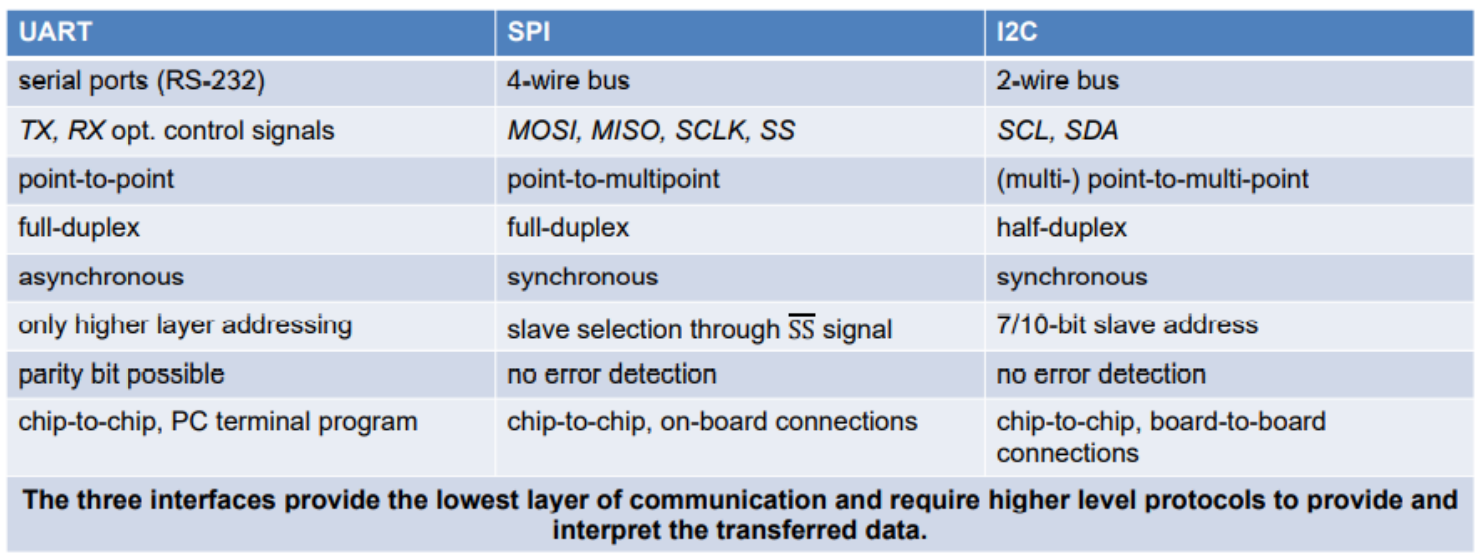
\includegraphics[width=\linewidth]{SDT_overview.png}
    \vspace{2mm}\\
    \textbf{SPI - Serial Peripheral Interface}
    \begin{itemize}
        \item Master/slave
        \item Synchronous full-duplex transmissions (MOSI, MISO)
        \item Selection of device through Slave Select (SS)
        \item no acknowledge, no error detection
        \item Clock signal (SCK) for synchronization: four mode $\rightarrow$ CPOL (clock polarity), CPHA (clock phase)
    \end{itemize}
    \vspace{2mm}

    \textbf{UART - Universal Asynchronous Receiver Transmitter} (Serial Interface)
    \begin{itemize}
        \item Transmitter and receiver use diverging clocks
        \item synchronization using start and stop bits $\rightarrow$ overhead
        \item longer connections require line drivers $\rightarrow$ RS-232/RS-485
    \end{itemize}
    \vspace{2mm}

    \textbf{I2C - Inter-Integrated Circuit}
    \begin{itemize}
        \item Synchronous half-duplex transmission (SCL, SDA)
        \item 7-bit slave addresses
        \item Acknowledge, error detection
        \item Clock signal (SCL) for synchronization
    \end{itemize}
\end{concept}

\begin{definition}{Single Master - Multiple Slaves}
    \begin{itemize}
        \item Master generates a common clock signal for all Slaves
        \item MOSI: From Master Output to all Slave Inputs
        \item MISO: From Master Input to all Slave Outputs $\rightarrow$ all slave outpuzs connected to single master input
        \item Slaves: Selectable by Slave Select (SS) signal
        \begin{itemize}
            \item Individual Select $\overline{SS1}$, $\overline{SS2}$, $\overline{SS3}$
            \item $\overline{SSx}$ = 1 $\rightarrow$ slave output MISOx is tri-state 
        \end{itemize}
    \end{itemize}
    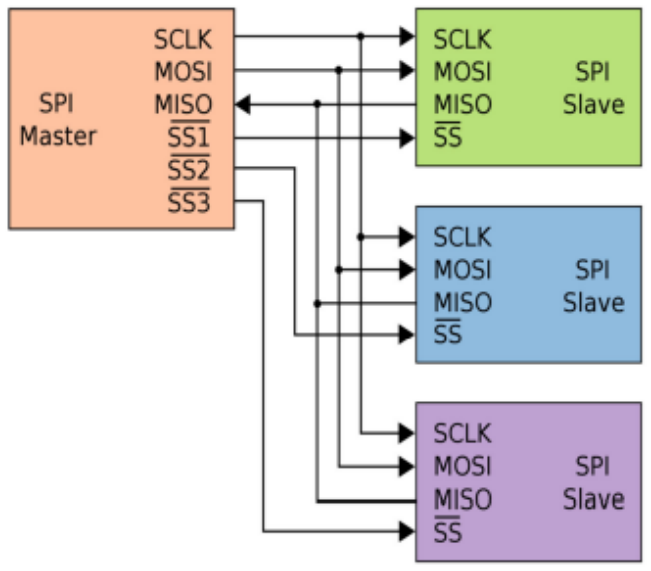
\includegraphics[width=\linewidth]{single_master_mult_slaves.png}
\end{definition}

\begin{formula}{Clock Polarity (CPOL) Clock Phase (CPHA)}
    \begin{itemize}
        \item \textbf{CPOL:} Clock Polarity
        \begin{itemize}
            \item 0: Clock is low in idle state
            \item 1: Clock is high in idle state
        \end{itemize}
        \item \textbf{CPHA:} Clock Phase
        \begin{itemize}
            \item 0: Data is sampled on the first edge of the clock
            \item 1: Data is sampled on the second edge of the clock
        \end{itemize}
    \end{itemize}
    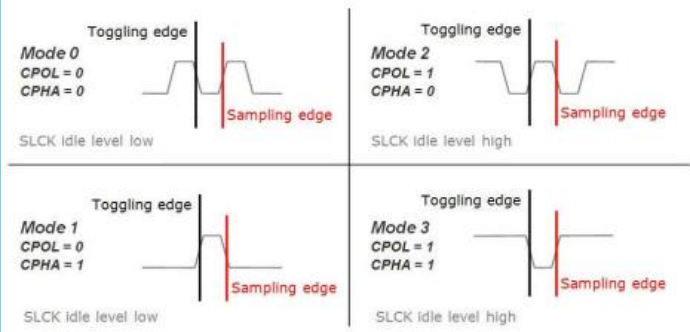
\includegraphics[width=\linewidth]{clockpolarity.png}
    \begin{itemize}
        \item TX provides data on \oq Toggling Edge\cq
        \item RX takes over data with \oq Sampling Edge\cq
    \end{itemize}
\end{formula}

\subsection{Serial Connection - SPI}

\begin{definition}{Properties of SPI}
    \begin{itemize}
        \item No defined addressing scheme
        \begin{itemize}
            \item Use of $\overline{SS}$ instead $\rightarrow$ KISS (Keep It Simple Stupid)
        \end{itemize}
        \item Transmission without receive acknowledge and error detection
        \begin{itemize}
            \item Has to be implemented in higher level protocols
        \end{itemize}
        \item Originally used only for transmission of single bytes
        \begin{itemize}
            \item $\overline{SS}$ deactivated after each byte
            \item Today also used for streams 
        \end{itemize}
        \item Data rate: Highly flexible as clock signal is transmitted
        \item No flow-control available
        \begin{itemize}
            \item Master can delay the next clock edge
            \item Slave can't influence the data rate
        \end{itemize}
        \item Susceptible to noise (spikes on clock signal)
    \end{itemize}
\end{definition}

\begin{example2}{SPI - Serial Peripheral Interface}\\
    Ein Prozessor (SPI Master) sendet das Byte 0x3D = 0011 1101\\
    Die Schnittstelle ist wie folgt konfiguriert:\\
    Mode = 3, CPOL = 1, CPHA = 1, MSB first\\
    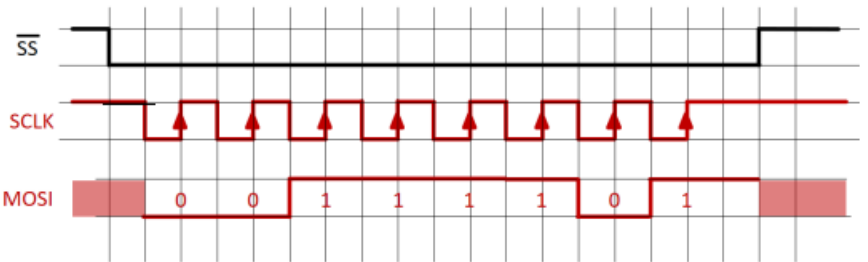
\includegraphics[width=\linewidth]{spi_example.png}
\end{example2}

\begin{concept}{Synchronizing Hardware and Software}
    \begin{itemize}
        \item TXE (TX Buffer Empty) $\rightarrow$ Software can write next TX Byte to SPI\_DR
        \item RXNE (RX Buffer Not Empty) $\rightarrow$ a byte has been received. Software can read it from SPI\_DR
        \item BSY (Busy) $\rightarrow$ Transmission in progress
    \end{itemize}
    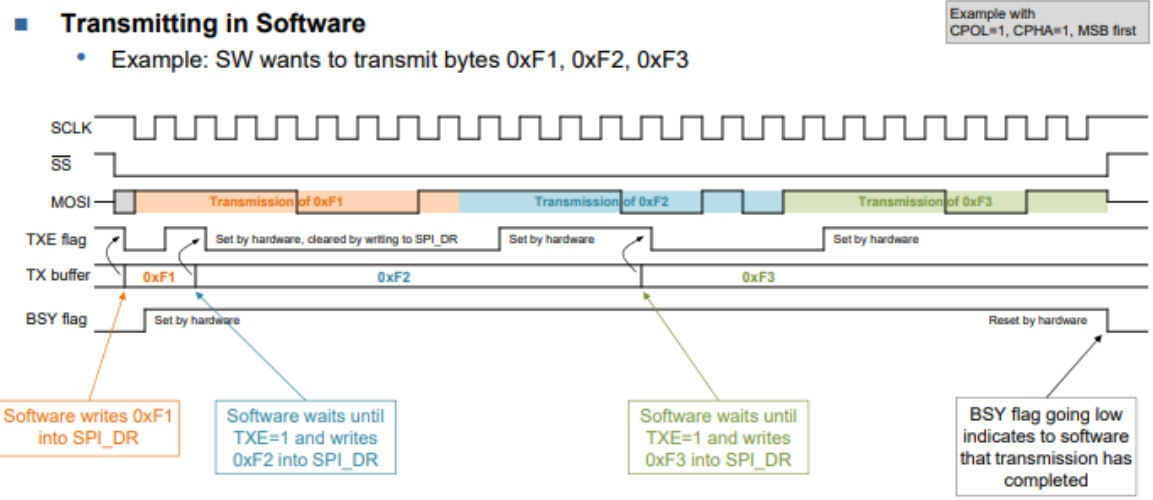
\includegraphics[width=\linewidth]{transmitting_spi.png}\\
    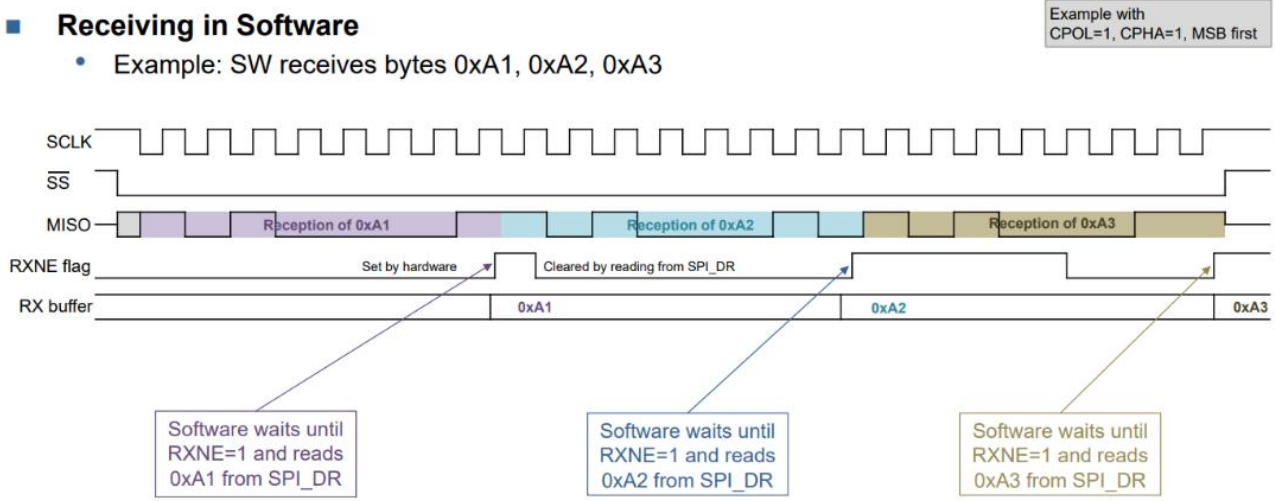
\includegraphics[width=\linewidth]{receiving_spi.png}
\end{concept}

\subsection{UART/I2C}

\begin{definition}{UART - Universal Asynchronous Receiver Transmitter}\\
    Connecting shift registers with diverging clock sources
    \begin{itemize}
        \item same target frequency
        \item different tolerances and divider ratios
        \item requires synchronization at start of each data item receiver
    \end{itemize}
    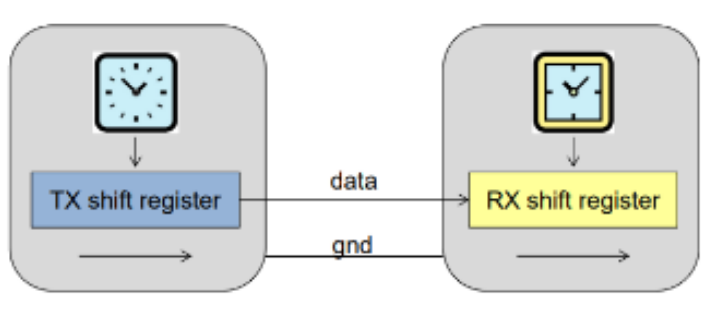
\includegraphics[width=\linewidth]{uart.png}
\end{definition}

\begin{concept}{UART Characteristics}
    \vspace{2mm}\\
    \textbf{synchronization}
    \begin{itemize}
        \item Each data item (5-8 bits) requires synchronization
    \end{itemize}
    \vspace{2mm}

    \textbf{Asynchronous data transfer}
    \begin{itemize}
        \item mismatch of clock frequencies in TX and RX
        \item requires overhead for synchronization $\rightarrow$ additional Bits
        \item requires effort for synchronization $\rightarrow$ additional Hardware
    \end{itemize}
    \vspace{2mm}

    \textbf{Advantages}
    \begin{itemize}
        \item Clock does not have to be transmitted
        \item transmission delays are automatically compensated
        \item no need for a common clock signal
    \end{itemize}
    \vspace{2mm}
    
    \textbf{on-board connections}
    \begin{itemize}
        \item signal levels are 3V or 5V with reference to ground
        \item off-board connections require strong output drivers
    \end{itemize}
\end{concept}

\section{Serial Data Transfer Exercises}

\subsection{UART Communication}

\begin{KR}{Analyzing UART Transmission}
\paragraph{Determine bit timing}
\begin{itemize}
    \item Calculate bit period (T) from baud rate: T = 1/baud\_rate
    \item Example: 19200 baud = 1/19200 s = 52.1 µs per bit
\end{itemize}

\paragraph{Identify frame structure}
\begin{itemize}
    \item Start bit: Always '0'
    \item Data bits: LSB first, typically 7 or 8 bits
    \item Parity bit: Optional, can be even, odd, mark ('1'), or space ('0')
    \item Stop bit(s): Always '1', can be 1, 1.5, or 2 bits
    \item Idle state: Line remains high ('1')
\end{itemize}

\paragraph{Calculate total frame time}
\begin{itemize}
    \item Add up all bits: Start bit + Data bits + Parity bit + Stop bits
    \item Multiply by bit period (T)
    \item Example: 8N1 (8 data bits, no parity, 1 stop bit) = 10 bits total
\end{itemize}

\paragraph{Calculate maximum throughput}
\begin{itemize}
    \item Divide baud rate by total number of bits per frame
    \item Example: 9600 baud, 8N1 format = 9600/10 = 960 bytes/second
\end{itemize}

\paragraph{Evaluate clock tolerance}
\begin{itemize}
    \item Maximum tolerable deviation is typically ±(0.5/n) where n is the number of bits from start bit to the last data bit
    \item Example: For 8 data bits, max deviation = ±(0.5/8.5) $\approx$ ±5.9\%
\end{itemize}
\end{KR}

\begin{example2}{UART Transmission Analysis}\\
For a UART transmission with 19,200 bits/s, 7 data bits, and one stop bit (no parity), draw the timing diagram for transmitting the ASCII characters "AC".

ASCII values:
\begin{itemize}
    \item 'A' = 0x41 = 100 0001b
    \item 'C' = 0x43 = 100 0011b
\end{itemize}

\tcblower
\paragraph{Solution:}
First, calculate the bit period:
\begin{itemize}
    \item T = 1/19200 s = 52.1 µs
\end{itemize}

For each character, the frame consists of:
\begin{itemize}
    \item 1 start bit (S) - always '0'
    \item 7 data bits (D) - LSB first
    \item 1 stop bit (E) - always '1'
\end{itemize}

Between frames, the line is idle (I) - high.

Frame for 'A' (0x41 = 100 0001b):
\begin{itemize}
    \item Start bit (S): 0
    \item Data bits (D), LSB first: 1, 0, 0, 0, 0, 0, 1
    \item Stop bit (E): 1
\end{itemize}

Frame for 'C' (0x43 = 100 0011b):
\begin{itemize}
    \item Start bit (S): 0
    \item Data bits (D), LSB first: 1, 1, 0, 0, 0, 0, 1
    \item Stop bit (E): 1
\end{itemize}

The timing diagram:
\begin{verbatim}
   I I S D D D D D D D E S D D D D D D D E I I I
   1 1 0 1 0 0 0 0 0 1 1 0 1 1 0 0 0 0 1 1 1 1 1
   <--------------'A'------------><--------------'C'------------->
\end{verbatim}

Each bit has a duration of T = 52.1 µs, so the total transmission time for both characters is:
\begin{itemize}
    \item 2 characters × 9 bits per character × 52.1 µs = 937.8 µs
\end{itemize}

The clock tolerance can be calculated as:
\begin{itemize}
    \item For 7 data bits: max deviation = ±(0.5/7.5) $\approx$ ±6.67\%
\end{itemize}
\end{example2}

\subsection{SPI Communication}

\begin{KR}{Analyzing SPI Communication}
\paragraph{Identify SPI mode}
\begin{itemize}
    \item Determine CPOL (Clock Polarity):
    \begin{itemize}
        \item CPOL=0: Clock idles low
        \item CPOL=1: Clock idles high
    \end{itemize}
    \item Determine CPHA (Clock Phase):
    \begin{itemize}
        \item CPHA=0: Data sampled on first edge (leading edge)
        \item CPHA=1: Data sampled on second edge (trailing edge)
    \end{itemize}
    \item Identify SPI mode from CPOL and CPHA:
    \begin{itemize}
        \item Mode 0: CPOL=0, CPHA=0
        \item Mode 1: CPOL=0, CPHA=1
        \item Mode 2: CPOL=1, CPHA=0
        \item Mode 3: CPOL=1, CPHA=1
    \end{itemize}
\end{itemize}

\paragraph{Draw timing diagram}
\begin{itemize}
    \item First, draw clock (SCLK) based on CPOL
    \item Draw chip select (SS\#) - active low
    \item Draw MOSI line with data from master to slave
    \item Draw MISO line with data from slave to master
    \item Indicate sampling edges based on CPHA:
    \begin{itemize}
        \item CPHA=0: Sample on rising edge if CPOL=0, falling edge if CPOL=1
        \item CPHA=1: Sample on falling edge if CPOL=0, rising edge if CPOL=1
    \end{itemize}
\end{itemize}

\paragraph{Calculate timing parameters}
\begin{itemize}
    \item Bit cell time = 1/clock\_frequency
    \item Frame time = (number\_of\_bits)/clock\_frequency
    \item Example: 8 bits at 100 kHz = 80 µs per frame
\end{itemize}
\end{KR}

\begin{example2}{SPI Timing Diagram Example}\\
Draw the timing diagram for an SPI transfer with:
\begin{itemize}
    \item Mode 3 (CPOL=1, CPHA=1)
    \item 8-bit data: MOSI = 0xA7, MISO = 0x37
    \item MSB first
    \item Clock frequency = 100 kHz
\end{itemize}
Mark all sampling edges on the diagram.

\tcblower
\paragraph{Solution:}
For Mode 3:
\begin{itemize}
    \item CPOL=1: Clock idles high
    \item CPHA=1: Data sampled on second edge (trailing edge)
    \item Sampling occurs on rising clock edges
\end{itemize}

Data values in binary:
\begin{itemize}
    \item MOSI: 0xA7 = 10100111
    \item MISO: 0x37 = 00110111
\end{itemize}

Bit cell time = 1/100 kHz = 10 µs

Timing diagram:
\begin{verbatim}
SS#   _|________________________________|_
          
SCLK  _|¯|_|¯|_|¯|_|¯|_|¯|_|¯|_|¯|_|¯|_|¯|_
          ^   ^   ^   ^   ^   ^   ^   ^
MOSI  ___|1|0|1|0|0|1|1|1|_________________
          
MISO  ___|0|0|1|1|0|1|1|1|_________________
\end{verbatim}

The arrows ($\wedge$) mark the sampling edges, which are the rising edges in Mode 3.

Total frame time = 8 bits × 10 µs = 80 µs.
\end{example2}

\subsection{I2C Communication}

\begin{KR}{Analyzing I2C Communication}
\paragraph{Identify I2C protocol elements}
\begin{itemize}
    \item Start condition: SDA falls while SCL is high
    \item Stop condition: SDA rises while SCL is high
    \item Data bit transfer: SDA stable while SCL is high
    \item Acknowledge (ACK): Receiver pulls SDA low during 9th clock cycle
    \item Not-acknowledge (NACK): SDA remains high during 9th clock cycle
\end{itemize}

\paragraph{Parse I2C frames}
\begin{itemize}
    \item First byte after start: 7-bit address + R/W bit
    \begin{itemize}
        \item R/W = 0: Write operation
        \item R/W = 1: Read operation
    \end{itemize}
    \item Check for ACK/NACK after each byte
    \item Data bytes follow (8 bits each)
    \item Master or slave can end transmission with STOP condition
\end{itemize}

\paragraph{Interpret timing diagram}
\begin{itemize}
    \item Examine SCL and SDA lines
    \item Identify start and stop conditions
    \item Group bits into bytes (8 bits + ACK/NACK)
    \item Determine if each byte is address or data
    \item Note the direction of data transfer
\end{itemize}
\end{KR}

\begin{example2}{I2C Communication Analysis}\\
Analyze the following I2C timing diagram and describe the transaction:

\begin{verbatim}
SCL  _____|¯¯¯|_|¯¯¯|_|¯¯¯|_|¯¯¯|_|¯¯¯|_|¯¯¯|_|¯¯¯|_|¯¯¯|_|¯¯¯|_|¯¯¯|...|¯¯¯|_|¯¯¯|_|¯¯¯|_|¯¯¯|_|¯¯¯|_|¯¯¯|_|¯¯¯|_|¯¯¯|_|¯¯¯|___
                     
SDA  ___\_|1|_|1|_|0|_|0|_|1|_|1|_|0|_|1|_|0|_\_|0|_|0|_|1|_|1|_|1|_|0|_|0|_|1|_/___
     Start                              ACK                 NACK  Stop
\end{verbatim}

\tcblower
\paragraph{Solution:}
The I2C transaction consists of:
\begin{enumerate}
    \item Start condition (SDA falls while SCL is high)
    \item First byte: 11001101 (data transmitted MSB first)
    \begin{itemize}
        \item This is the address byte: 1100110 (0x66) with R/W bit = 1 (read operation)
        \item Followed by an ACK (SDA pulled low during 9th clock cycle)
    \end{itemize}
    \item Second byte: 00111001 (data received from slave)
    \begin{itemize}
        \item This is data: 0x39 or 0x9C (depending on bit order interpretation)
        \item Followed by a NACK (SDA remains high during 9th clock cycle)
        \item NACK indicates that the master does not want to receive more data
    \end{itemize}
    \item Stop condition (SDA rises while SCL is high)
\end{enumerate}

The complete transaction is:
\begin{itemize}
    \item Master initiates communication with device at address 0x66
    \item Master requests to read from the device (R/W=1)
    \item Device acknowledges (ACK)
    \item Device sends one data byte (0x39 or 0x9C)
    \item Master signals end of transfer with NACK
    \item Master terminates communication
\end{itemize}
\end{example2}

\subsection{Protocol Comparison and Selection}

\begin{KR}{Selecting the Appropriate Serial Protocol}
\paragraph{Understand protocol characteristics}
\begin{itemize}
    \item \textbf{UART:}
    \begin{itemize}
        \item Point-to-point, full-duplex
        \item Asynchronous, no shared clock
        \item Simple wiring (2-3 wires)
        \item Moderate speed (up to ~5 Mbps)
    \end{itemize}
    \item \textbf{SPI:}
    \begin{itemize}
        \item Master-slave, full-duplex
        \item Synchronous with shared clock
        \item Multiple wires (MOSI, MISO, SCLK, SS)
        \item High speed (up to 50+ Mbps)
    \end{itemize}
    \item \textbf{I2C:}
    \begin{itemize}
        \item Multi-master, multi-slave
        \item Synchronous with shared clock
        \item Two wires (SCL, SDA)
        \item Medium speed (100 kbps, 400 kbps, up to 5 Mbps)
    \end{itemize}
\end{itemize}

\paragraph{Consider application requirements}
\begin{itemize}
    \item \textbf{Distance:}
    \begin{itemize}
        \item UART with RS-232 levels for longer distances
        \item SPI and I2C typically for on-board connections
    \end{itemize}
    \item \textbf{Speed:}
    \begin{itemize}
        \item SPI for highest speed requirements
        \item I2C for moderate speed with fewer pins
        \item UART for simpler, moderate speed connections
    \end{itemize}
    \item \textbf{Number of devices:}
    \begin{itemize}
        \item I2C for many devices on shared bus
        \item SPI for multiple devices but requires separate SS line for each
        \item UART typically for point-to-point (multiple UARTs needed for multiple devices)
    \end{itemize}
\end{itemize}

\paragraph{Evaluate protocol overhead}
\begin{itemize}
    \item \textbf{UART:}
    \begin{itemize}
        \item Start, stop, and optional parity bits
        \item Requires accurate clock timing
    \end{itemize}
    \item \textbf{SPI:}
    \begin{itemize}
        \item Minimal protocol overhead
        \item No addressing or acknowledgment
    \end{itemize}
    \item \textbf{I2C:}
    \begin{itemize}
        \item Start/stop conditions, addressing, and acknowledgment
        \item Higher protocol overhead but better error detection
    \end{itemize}
\end{itemize}

\paragraph{Consider hardware support}
\begin{itemize}
    \item Check if target microcontroller has hardware support for chosen protocol
    \item Consider available pins and alternate functions
    \item Evaluate available software libraries and drivers
    \item Consider power requirements (I2C has pull-up resistors that consume power)
\end{itemize}
\end{KR}

\begin{example2}{Serial Protocol Selection}\\
Select the most appropriate serial protocol for each of the following applications:
\begin{enumerate}
    \item A system needs to connect a microcontroller to three temperature sensors. The sensors are low-cost devices that should be replaceable without redesigning the PCB. Data rate requirement is low.
    \item A data acquisition system needs to transfer large amounts of data from an ADC to a microcontroller at 20 Mbps.
    \item A microcontroller needs to communicate with a PC via USB port.
    \item A control system needs to connect to four different devices at varying distances up to 30 meters in an electrically noisy industrial environment.
\end{enumerate}
\paragraph{Solution:}

1. \textbf{I2C is most appropriate for the temperature sensors:}
   \begin{itemize}
     \item Multiple devices (three sensors) can be connected to the same two wires
     \item Each sensor has a unique address, making them individually addressable
     \item Low data rate requirement is well within I2C capabilities
     \item Sensors can be replaced without changing connections (as long as addresses are configured properly)
     \item Reduced pin count (only SCL and SDA) simplifies PCB design
   \end{itemize}
   \vspace{2mm}
2. \textbf{SPI is most appropriate for the high-speed ADC:}
   \begin{itemize}
     \item 20 Mbps data rate exceeds practical I2C speeds and most UART configurations
     \item SPI can easily handle 20+ Mbps with direct hardware support
     \item SPI's full-duplex capability allows simultaneous control and data transfer
     \item Minimal protocol overhead maximizes throughput for large data amounts
     \item Hardware-based chip select ensures proper timing for ADC operations
   \end{itemize}
   \vspace{2mm}
3. \textbf{UART is most appropriate for PC communication:}
   \begin{itemize}
     \item UART is the typical protocol used with USB-to-serial converter chips
     \item Simple point-to-point connection is sufficient for PC communication
     \item Standard baudrates (9600, 115200, etc.) are well-supported by PC software
     \item No need for extra clock signals simplifies interfacing with USB adapters
     \item Asynchronous nature accommodates timing differences between systems
   \end{itemize}
   \vspace{2mm}
4. \textbf{RS-485 (based on UART) is most appropriate for the industrial control system:}
   \begin{itemize}
     \item RS-485 extends UART to longer distances (up to 1200m)
     \item Differential signaling provides excellent noise immunity in industrial environments
     \item Multi-drop capability allows connection to four devices on a single bus
     \item Higher voltage levels offer better signal integrity over 30m distances
     \item Various data rates possible depending on cable length (up to 10 Mbps at shorter distances)
     \item Industry standard protocol with wide hardware support
   \end{itemize}
\end{example2}
    